\documentclass[ucs,9pt]{beamer}
% \documentclass[ucs,9pt,handout]{beamer}
\setbeamercovered{transparent}
\newcommand{\semitransp}[2][35]{\color{fg!#1}#2}

\usepackage[utf8x]{inputenc} % Set input encoding to UTF-8.
\usepackage[english]{babel} % Set language.
\usepackage{nicefrac}
\usepackage{courier}

% activate KDE theme
\usepackage{KDE/beamerthemeKDE}
\usepackage{tikz}
\usepackage{multicol}
\usepackage{listings}

\title[Automotive ECUs with Yocto]{Short Dive into Building\newline Automotive ECUs with Yocto}
\subtitle{First Steps into Yocto}
\author{Andreas Cord-Landwehr}
\date{\textnormal{August 12th, 2018\\[\medskipamount] Akademy 2018, Vienna}}

\newcommand{\KDEemail}{cordlandwehr@kde.org}
% \newcommand{\KDEweb}{https://talks.cord-landwehr.de}
% \newcommand{\KDEaffiliation}{KDE Developer}
% % %

\lstset{ %
  language=C++,
  backgroundcolor=\color{KDEgray4},
  basicstyle=\footnotesize\ttfamily,
  breakatwhitespace=false,
  breaklines=true,
  captionpos=b,
  commentstyle=\color{KDEgreen},
  escapeinside={\%*}{*)},
  extendedchars=true,
  frame=single,
  keywordstyle=\color{KDEblue},
  language=Prolog,
  numbers=left,
  numbersep=5pt,
  numberstyle=\tiny\color{lightgray},
  rulecolor=\color{lightgray},
  showspaces=false,
  showstringspaces=false,
  showtabs=false,
  stepnumber=1,
  stringstyle=\color{KDEorange},
  tabsize=2,
  title=\lstname,
  morekeywords={Item,import,not,\},\{,Q_SIGNALS,public,Q_OBJECT,virtual,NOTIFY,Q_NULLPTR,Q_DISABLE_COPY,Q_DECL_OVERRIDE},
  deletekeywords={time}
}

%TikZ Definitions
\usetikzlibrary{arrows}
\usetikzlibrary{fit}
\usetikzlibrary{shadows}
\usetikzlibrary{patterns}
\usetikzlibrary{matrix}
\usetikzlibrary{shapes}
\usetikzlibrary{calc}
\usetikzlibrary{decorations.pathmorphing}
\usetikzlibrary{positioning}
\usetikzlibrary{backgrounds}
\usetikzlibrary{decorations}
\usetikzlibrary{decorations.pathreplacing}

\usepackage[variablett]{lmodern}

\newcommand*{\eswap}[3]{#1:[#2\rightarrow#3]}

\begin{document}
\maketitle

\begin{frame}
    {Introduction}
    {About Me \& the Talk}

    \begin{textblock*}{.3\paperwidth}[1,0](\paperwidth-1.5em,1em)%
        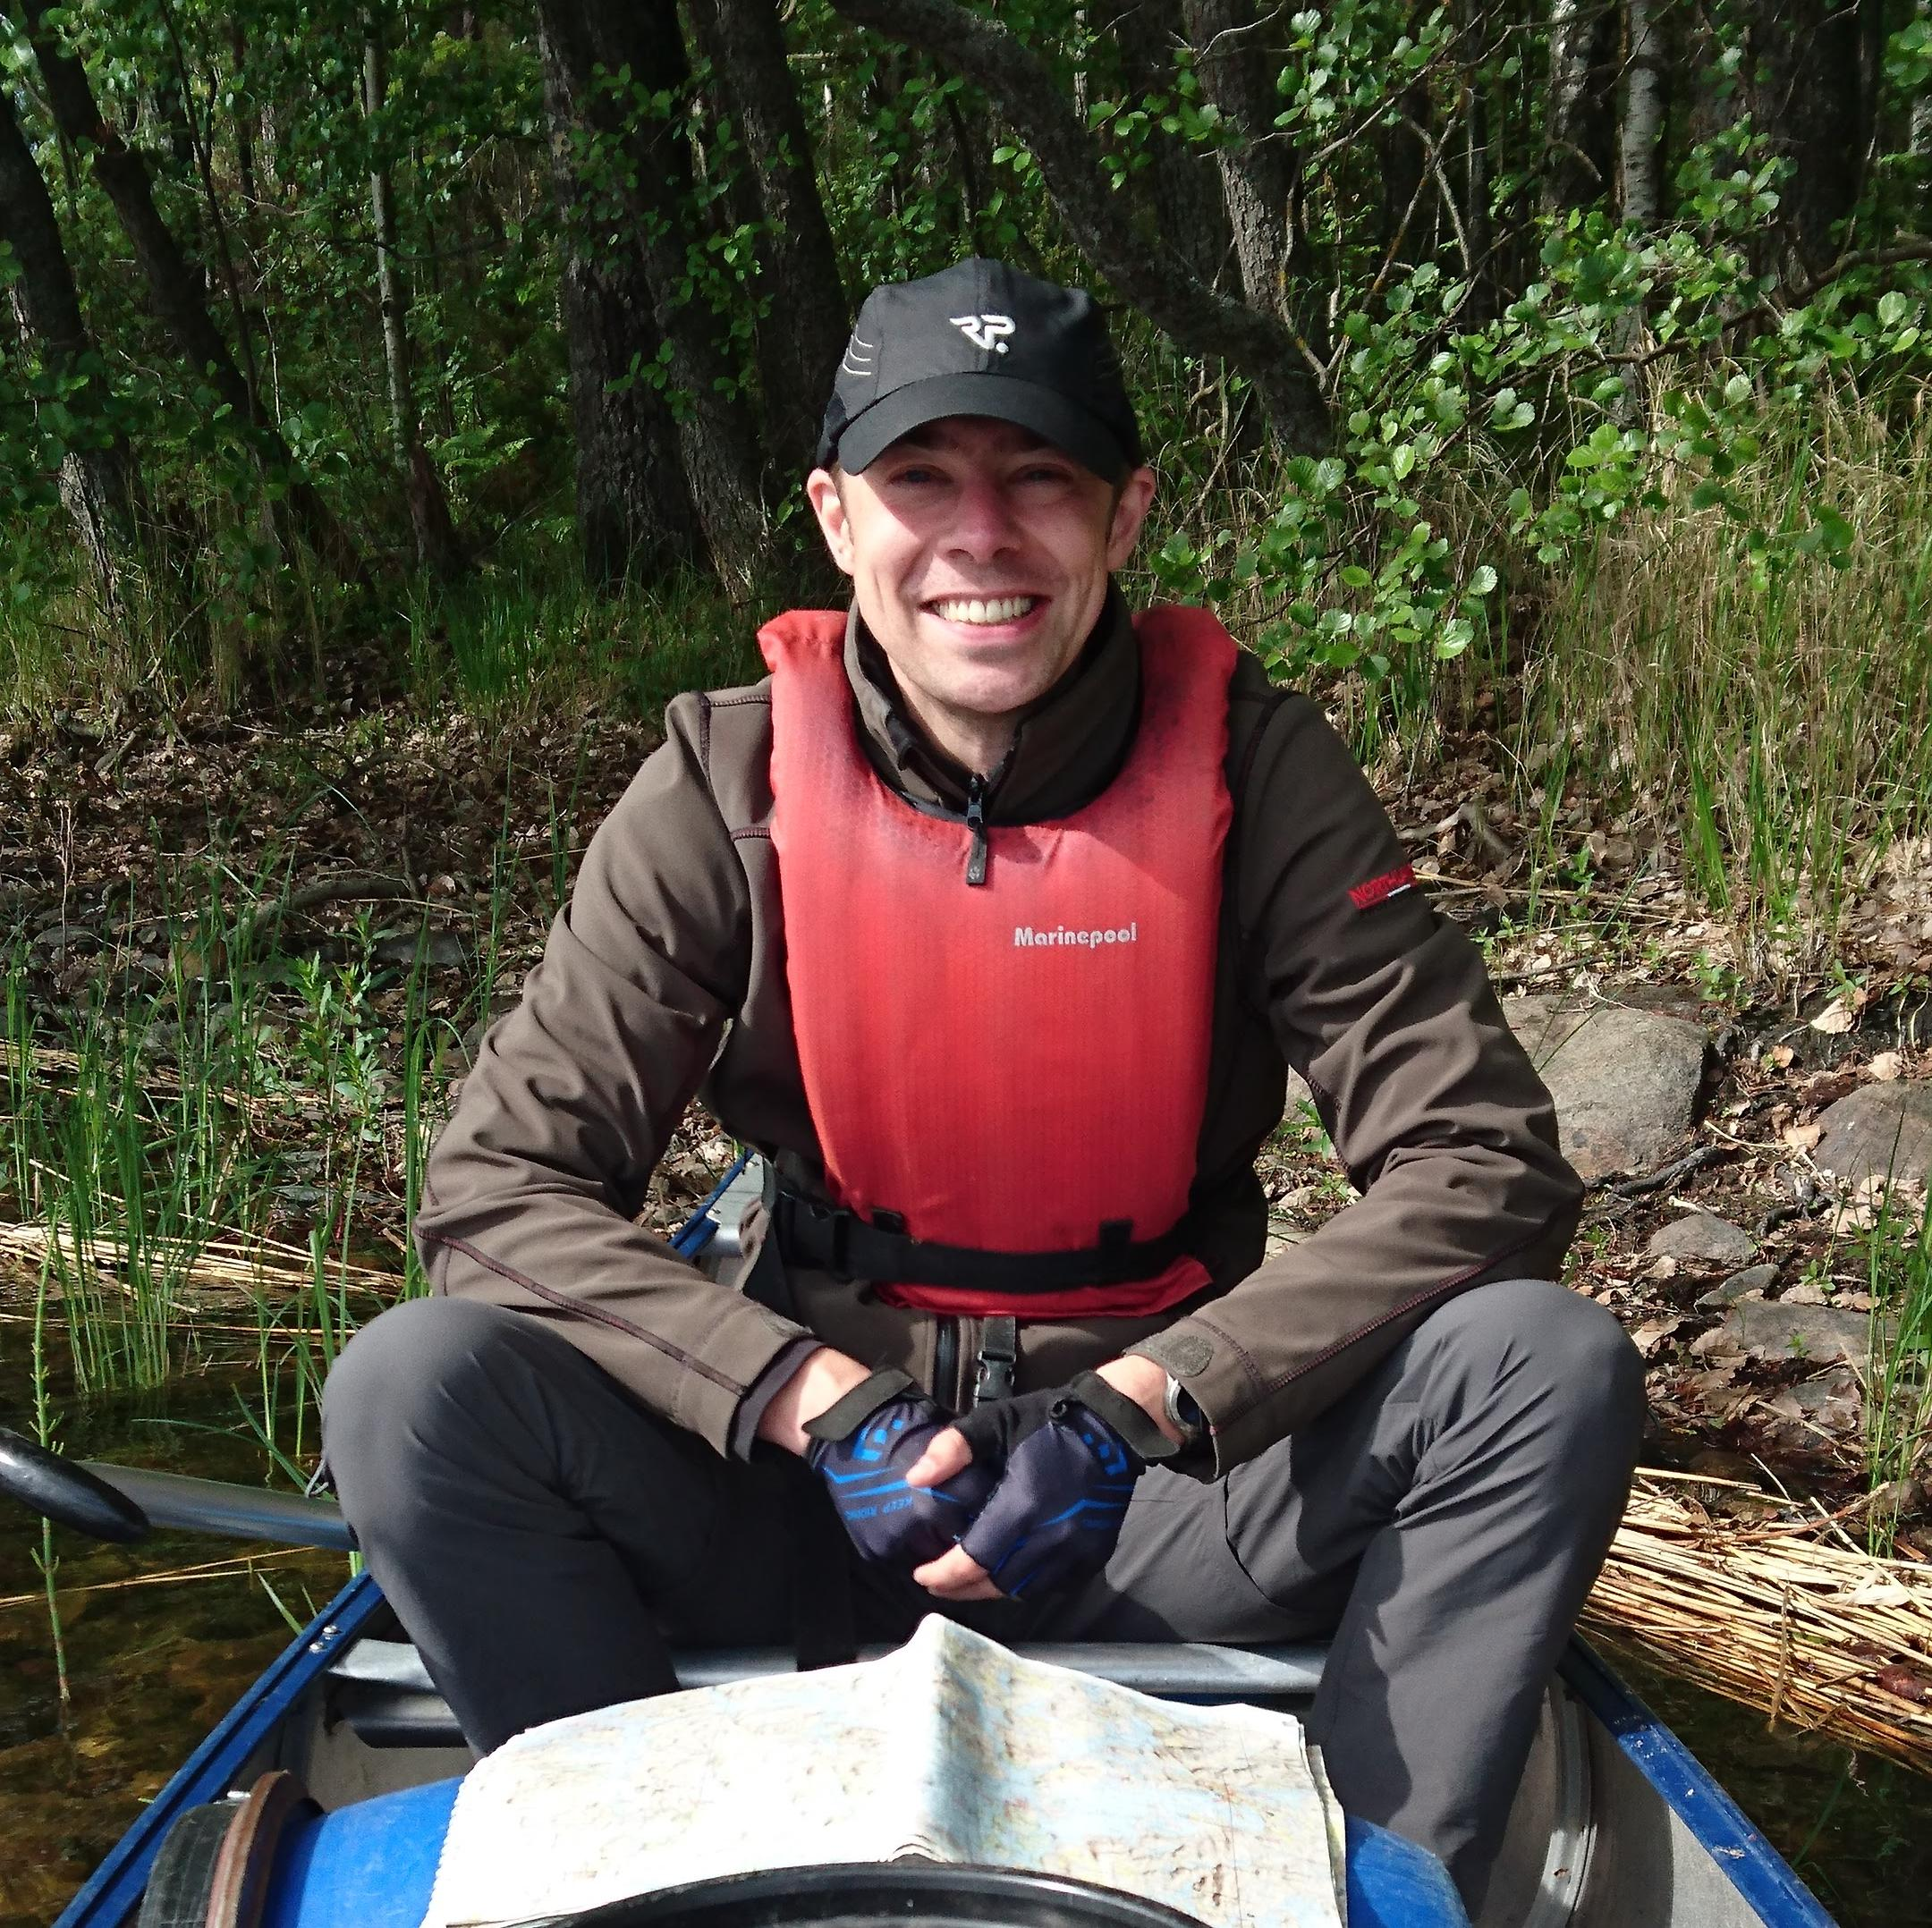
\includegraphics[width=\linewidth]{images/me}
    \end{textblock*}%

    \textbf{About Me}
    \begin{itemize}
        \item IRC-nick: CoLa
        \item KDE developer since 2010; mostly KDE-Edu
        \item did PhD in algorithmic game theory
        \item now working as software developer at\newline
            CLAAS E-Systems and creating terminals for big agriculture machines
        \begin{itemize}
            \item could be called ``enterprise embedded'' development
            \item key areas: Qt, C++, embedded Linux, Yocto
            \item several Yocto-based ARM devices are at my desk
        \end{itemize}
    \end{itemize}
    \bigskip

    \textbf{The Next 23 Minutes:}
    \begin{enumerate}
        \item Introduction into Yocto
        \item Using Yocto to build images and SDKs
        \item How to create KDE-power devices with Yocto
    \end{enumerate}
\end{frame}


\section{Part 1: Yocto Basics}

\begin{frame}
    {Embedded Devices in Scope of this Talk}

    \begin{center}
        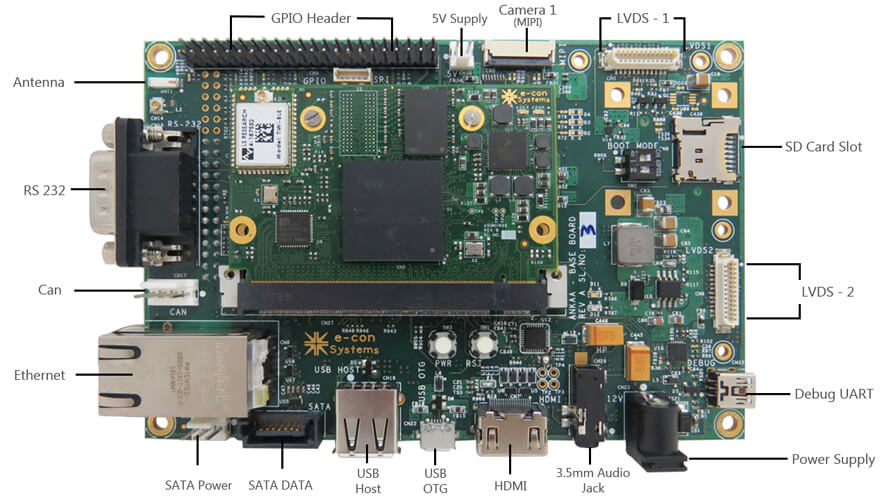
\includegraphics[width=.5\paperwidth]{images/example-board}\\
        \tiny source: https://www.e-consystems.com
    \end{center}

    \begin{description}
        \item [custom hardware:] purpose-tailored hardware, e.g.\ ARM CPU, CAN interface, 100BaseT1 Ethernet, NAND memory, GPIOs for different purposes
        \item [hardware evolves:] hardware and software are often developed at the same time and only a limited number of prototype devices is available
        \item [custom flashing process:] devices must be flashed by developers, updated by technicians on field and provisioned at end of the manufacturing line
        \item [cross-building:] hardware architecture different to x86 development machine
        \item [operating system:] in this talk we only look at Linux (note: no hard real-time)
    \end{description}
\end{frame}

\begin{frame}
    {The Basic Issue: Creating a System Image}

    \begin{textblock*}{.2\paperwidth}[1,0](\paperwidth-1em,1em)%
        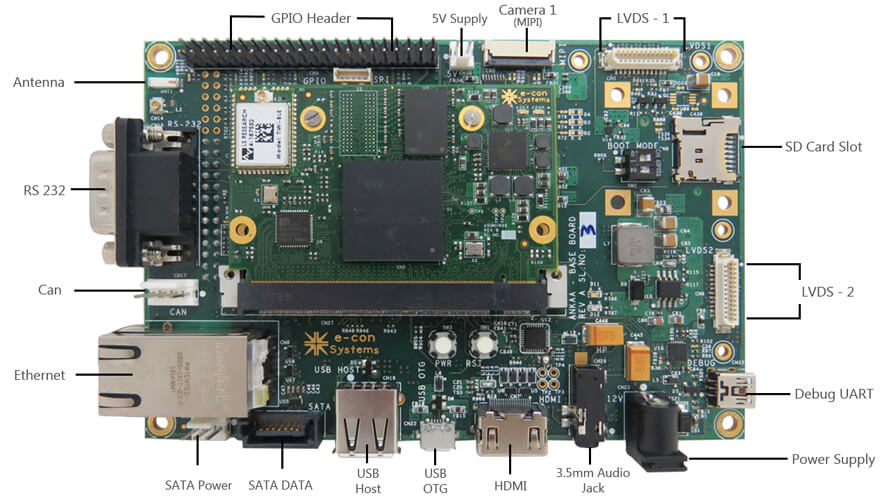
\includegraphics[width=\linewidth]{images/example-board}
    \end{textblock*}%


    \begin{block}{Issue Statement}
    For a given target device, we want to generate a system image:
    \begin{itemize}
        \item image is a root file-system that is {\color{KDEblue}ready to be flashed} to persistent memory
        \item image contains applications and libraries that {\color{KDEblue}work on target device's architecture}
        \item image generation is {\color{KDEblue}reproduceable and well-definend} (= no magic happens)
        \item image shall be {\color{KDEblue}created on an x86 developer machine}
    \end{itemize}
    \end{block}
    \bigskip\par
    In the remainder of this talk, I will outline how Yocto attempts to solve this task.
\end{frame}


\begin{frame}
    {About the Yocto Project}

    \begin{textblock*}{.2\paperwidth}[1,0](\paperwidth,0pt)%
        
\includegraphics[width=\linewidth]{images/yocto-logo}
    \end{textblock*}%

    \begin{block}{}
        \emph{The Yocto Project is an open source collaboration project that provides templates, tools and methods to help you create custom Linux-based systems for embedded and IOT products, regardless of the hardware architecture.}
        \\
        \hfill\tiny https://www.yoctoproject.org/about/
    \end{block}

    This means that Yocto\ldots
    \begin{enumerate}
        \item strives for being an ecosystem that makes device creation simple
        \item aims to provide all tools needed for doing this job
        \item ensures reusability and vendor independence by defining general rules
    \end{enumerate}
    \medskip
    \pause

    \textbf{Basic Notions:}
    \begin{description}
        \item [Recipe:] build and packaging instructions for compiling a source code package
        \item [Layer:] set of recipes and/or modifications of other recipes
        \item [Image:] complete root file system that is flashed onto a device
        \item [SDK:] set of cross-compiled libraries, header files and all cross-compilation tools needed to cross-compile code for a target device
    \end{description}
    \medskip
    %REMARK: move content up
\end{frame}

\begin{frame}
    {Building Block 1: OpenEmbedded-Core}

    \begin{textblock*}{.1\paperwidth}[1,0](\paperwidth-1em,1em)%
        
\includegraphics[width=\linewidth]{images/oe-logo}
    \end{textblock*}%

    \begin{block}{Yocto \& OpenEmbedded}
        \begin{itemize}
         \item OpenEmbedded is a build automation framework and cross-compile environment
         \item OpenEmbedded community was formally established in 2003; Yocto in 2010
         \item Yocto uses and co-maintains OpenEmbedded tools (BitBake, OE-Core)
        \end{itemize}
    \end{block}
    \pause

    \textbf{OpenEmbedded-Core = metadata \& build instructions}
    \begin{itemize}
        \item defines how basic tasks are performed (reused in recipes)
        \begin{enumerate}
            \item download source code
            \item configure source code
            \item setup build dependencies
            \item compile source code with the respective build system (CMake, QMake, Make\ldots)
            \item populate cross-building sysroot and create packages
            \item perform QA checks
        \end{enumerate}
        \item provides a big initial set of recipes for core libraries and applications
        \item supported platforms: ARM, MIPS, PowerPC, x86, QEMU
        \item repository: \url{http://git.openembedded.org/openembedded-core/}
    \end{itemize}
\end{frame}

\begin{frame}[fragile]
    {Building Block 2: BitBake}

    \begin{textblock*}{.25\paperwidth}[1,0](\paperwidth-1em,1em)%
        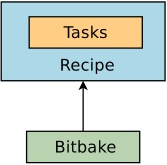
\includegraphics[width=\linewidth]{images/bitbake-definition}
    \end{textblock*}

    \textbf{BitBake = build system}
    \begin{itemize}
%         \item Python based build scheduler
        \item BitBake recipes specify how a particular package is built\\
            (by using basic OE-Core tasks)
        \item overall BitBake execution:
        \begin{enumerate}
            \item parses all available layers and their recipes
            \item prepares build tools and cross-build tools by configuring their environments
            \item schedules all basic tasks of all to be built packages by their defined dependencies (e.g. first download, then configure, then build; e.g. first build \texttt{qtbase} then \texttt{karchive})
            \item performs the specified basic tasks
        \end{enumerate}
        \item BitBake configuration consists of two parts:
        \begin{enumerate}
            \item environment configuration that is sourced by a script
            \item a folder \texttt{conf/} in the build directory that contains list of all layers (\texttt{bblayers.conf}) and build machine specific general configuration (\texttt{local.conf})
        \end{enumerate}
        \item repository: \url{http://git.openembedded.org/bitbake/}
    \end{itemize}
\end{frame}

\begin{frame}
    {Building Block 3: Poky}

    \begin{textblock*}{.1\paperwidth}[1,0](\paperwidth-1em,1em)%
        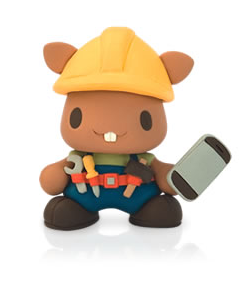
\includegraphics[width=\linewidth]{images/poky-beaver}
    \end{textblock*}%

    \textbf{Poky = reference \& quick-start distro}
    \begin{itemize}
        \item reference distribution of the Yocto Project
        \item contains BitBake: build system, task scheduler and executor
        \item contains metadata (global definitions, build logic, packaging, etc.):
        \begin{enumerate}
            \item OpenEmbedded-Core (OE-Core)
            \item Yocto Project-specific metadata (meta-yocto)
            \item Yocto Project-specific board support package (meta-yocto-bsp)
        \end{enumerate}
        \item Repository: \url{https://git.yoctoproject.org/cgit/cgit.cgi/poky/}
    \end{itemize}
    \bigskip

    Poky contains everything to start a new project or to be used as a blueprint.
\end{frame}

\begin{frame}
    {SDKs for your Yocto Image}

    \begin{block}{The Need for SDKs}
    \begin{itemize}
        \item building Yocto is complex and extremly time \& space consuming
        \item split responsibilities in a team: development vs.\ integration
        \item in industry, you might not want to disclose your source codes or build configuration to contractors
    \end{itemize}
    \end{block}
    \smallskip
    \par
    \textbf{Yocto's Standard SDK}
    \begin{itemize}
        \item allows compiling for target device without building the Yocto system first
        \item can be generated alongside with image (and ALWAYS must be ABI compatible with image)
        \item is a self-extracing (gigantic) shell script
        \item contains all needed cross-building tools and cross-built libraries
        \item can be integrated with your IDE (e.g. KDevelop, QtCreator)
        \item simply generate with: \texttt{bitbake -c do\_populate\_sdk}
    \end{itemize}
\end{frame}

\section{Part 2: Using Yocto}

\begin{frame}
    {Contents of a Typical Yocto System}

    \vspace{-1em}
    \begin{center}
    \includegraphics[width=.6\linewidth]{images/yocto-structure}
    \end{center}
    \begin{itemize}
        \item always needed: OE-Core, BitBake
        \item distribution: Poky or some custom distribution
        \item board support package (e.g. meta-ti, meta-fsl-arm)
        \item custom layers with your own recipes (e.g. meta-kf5)
    \end{itemize}
\end{frame}

\begin{frame}
    {KF5-powered Devices with Yocto: meta-kf5 \& meta-kde}

    Additional layers can bring additional libraries/applications to the Yocto world:
    \medskip

    \textbf{meta-kf5}
    \begin{itemize}
        \item provides build recipes for latest release of KF5
        \item provides all non-standard dependency recipes
        \item can easily be integrated into any (recent) Yocto project
        \item Repository: \url{https://cgit.kde.org/yocto-meta-kf5.git/}\\
            $\rightarrow$ thanks to Johan Thelin \& Volker Krause
    \end{itemize}

    \textbf{meta-kde}
    \begin{itemize}
        \item all recipes for building a full Plasma Desktop
        \item Repository: \url{https://cgit.kde.org/yocto-meta-kde.git/}\\
            $\rightarrow$ again, thanks to Volker!
    \end{itemize}
\end{frame}

\begin{frame}
    {And now?!}
    {How to start with Yocto and KF5?}

    This talk has (by far) not enough time to do that, but I would start as follows:

    \begin{enumerate}
        \item start with the Yocto quick start guide, setup your system and try with QEMU:\\
            \url{https://www.yoctoproject.org/docs/2.5/brief-yoctoprojectqs/brief-yoctoprojectqs.html}
        \item get a real development device (e.g. Raspberry, BeagleBone, i.MX6) and run your test system there\\
            $\rightarrow$ you will need a BSP layer for that\dots
        \item integrate \texttt{meta-qt5} and run a simple full-screen QML test application (or a console application, if you do not have a display)
        \item integrate \texttt{meta-kf5} and (if you want) \texttt{meta-kde}
    \end{enumerate}

\end{frame}


\begin{frame}
    {Further Reading \& References}
    \begin{itemize}
        \item Yocto Project Documentation\\
            \url{https://www.yoctoproject.org/docs/}
        \item BitBake User Manual\\
            \url{https://www.yoctoproject.org/docs/2.5/bitbake-user-manual/bitbake-user-manual.html}
        \item Yocto Reference Manual
            \url{https://www.yoctoproject.org/docs/2.5/ref-manual/ref-manual.html}
        \item OpenEmbedded Wiki\\
            \url{http://www.openembedded.org/wiki/Main_Page}
        \item Qt for Embedded\\
            \url{http://doc.qt.io/qt-5/embedded-linux.html}
    \end{itemize}
\end{frame}

\KDElastframe

\section{Appendix}
\begin{frame}[fragile]
    {Recipe Example}

    \begin{example}{}
    \hspace{1em}\begin{minipage}{.95\linewidth}
    \begin{lstlisting}[caption=attica\_5.48.0.bb,language=Python]
DESCRIPTION = "Attica"
HOMEPAGE = "https://api.kde.org/frameworks/attica/html/index.html"
LICENSE = "LGPL-2.1"
LIC_FILES_CHKSUM = "file://COPYING;md5=be254b9345b1c2ff33e1a6a96768f2fb"
PR = "r0"
DEPENDS = "qtbase"
SRC_URI = "git://anongit.kde.org/attica;nobranch=1"
S = "${WORKDIR}/git"
SRCREV = "v5.48.0"
inherit cmake_kf5
    \end{lstlisting}
    \end{minipage}
    \end{example}
\end{frame}


\begin{frame}[fragile]
    {Building Block 2 (ADD): BitBake Configuration}

    \begin{textblock*}{.25\paperwidth}[1,0](\paperwidth-1em,1em)%
        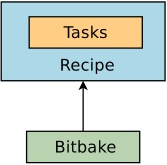
\includegraphics[width=\linewidth]{images/bitbake-definition}
    \end{textblock*}%

    A script with all varaibles needed by BitBake must be \emph{sourced}:
\begin{verbatim}
    source oe-init-build-env
\end{verbatim}

    Will move you in a \texttt{build} folder, where all commands can be run.
    All local configuration must be in a folder named \texttt{conf}
\begin{verbatim}
build/
    |-- conf
        |-- bblayers.conf
        |-- local.conf
\end{verbatim}

    Edit your \texttt{bblayers.conf} with all needed layers.
\end{frame}

\begin{frame}[fragile]
    {Building Block 2 (ADD): BitBake Machine}

    \begin{textblock*}{.25\paperwidth}[1,0](\paperwidth-1em,1em)%
        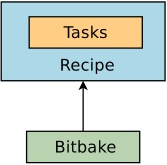
\includegraphics[width=\linewidth]{images/bitbake-definition}
    \end{textblock*}%

    Edit \texttt{local.conf} with your \texttt{MACHINE} and \texttt{DISTRO}
    \begin{itemize}
        \item \texttt{MACHINE}: describes your hardware.\\ Can find it under specific layers: BSP layers. Look at \texttt{conf/machine/} folders.
        \begin{itemize}
            \item poky: beaglebone, x86, x86-64
            \item meta-ti: beagleboard, pandaboard, \dots
            \item meta-fsl-arm: imx23, imx28, imx6, imx7,\dots
            \item meta-atmel: at91*, sama5d*
        \end{itemize}
        \item \texttt{DISTRO}: represents the top-level configuration that will apply to every build. It will include tools needed to use your hardware: compiler, libc, etc. + some specific variables; look at \texttt{conf/distro/} folders:
        \begin{itemize}
            \item poky: poky, poky-tiny, \dots
            \item meta-angstrom: angstrom
        \end{itemize}
    \end{itemize}
    Notice that \texttt{local.conf} is only for the local workstation!\\
    Avoid changes directly in \texttt{local.conf} (or only for test purposes; except for some variables such as MACHINE and DISTRO.
\end{frame}


\end{document}
